
\documentclass[conference]{IEEEtran}
% *** CITATION PACKAGES ***
%
\usepackage{cite}

% *** GRAPHICS RELATED PACKAGES ***
%
\usepackage[pdftex]{graphicx}
\graphicspath{./figures/}

% *** SUBFIGURE PACKAGES ***
%\ifCLASSOPTIONcompsoc
%  \usepackage[caption=false,font=normalsize,labelfont=sf,textfont=sf]{subfig}
%\else
%  \usepackage[caption=false,font=footnotesize]{subfig}
%\fi

\usepackage{url}


\begin{document}

\title{Clarifying the MM architecture}


% author names and affiliations
% use a multiple column layout for up to three different
% affiliations
\author{\IEEEauthorblockN{Alexis Jacq}

}



\maketitle

\IEEEpeerreviewmaketitle



\section{Remind of the framework}
\subsection{Justification of the approach}

A first intuition for mutual modelling is to assume that all agents have the same basic architecture. In~\cite{breazeal2006using}, Breazeal show a MM-based reasoning where the robot uses its own architecture to model other agents. We can imagine a second level of modelling where the robot recursively attribute to other agents the mutual modelling ability. But that creates an infinite recursive loop: the agent then models the robot that models the agent etc. Another reason to avoid a recursive approach is that different agent must have different behaviours: in similar situations, they will not necessary take similar decisions. 

We propose a different approach of modelling, where we define two orders of agent's model: the \textit{first-order-agents} concern direct representations of agents by the robot (for example the child), while the \textit{second-order-agents} concern the representation of agents by agents (for example the robot-perceived-by-the-child). 
To model second-order-agent like the robot-perceived-by-the-child will help to model how the child perceives the robot, e.g. to make sure the child understand that the robot is learning from his demonstrations. 
We can as well define \textit{$n^{\textit{th}}$-order} agents with higher level of theory of mind. But taking into account high levels of mutual modelling would be difficult to process in real time. Unlike the epistemic logic, our proposed framework will not take into account infinite regress~\cite{clark1991grounding} of mutual modelling.

\subsection{Notations}
$M_\textit{AB}$ stands for the model (built by the robot) of the agent B perceived by the agent A. As said above, we limit our approach to 1st and 2nd order of modelling. In a 2-agents interaction (the child and the robot) we will focus on 3 agent's models: $M_\textit{C}$ (the model of the child), $M_\textit{R}$ (the model of the robot) and $M_\textit{CR}$ (the robot perceived by the child). I would be also interesting to study $M_\textit{CC}$, the model of the child perceived by himself in order to play with his self-confidence. But detecting differences between $M_\textit{C}$ and $M_\textit{CC}$ seems difficult with the current abilities of the robot. 

As models are dynamic, $M_\textit{A}^t$ represent the model of an agent A at time $t$.

\section{Mutual understanding}
Given those three models ($M_\textit{R}$, $M_\textit{C}$ and $M_\textit{CR}$) the robot must be able to detect miss-understandings. Humans~\cite{suzuki2015neural} (and monkeys~\cite{haroush2015neuronal}), keep a mutual understanding with others by predicting their behaviour. A bio-inspired idea would be to make a prediction of $\hat{M}_\textit{C}^{t+1}$ and to estimate an error $E\left[\hat{M}_\textit{C}^{t};M_\textit{C}^{t}\right]$. In order to detect if the child understand the robot, the intuitive way is not to make a prediction, but to use the differences between $M_\textit{R}$ and $M_\textit{CR}$. For that, the same error function can be used: $E\left[M_\textit{R}^{t};M_\textit{CR}^{t}\right]$.

\section{Structure and dynamic of the models}
Each model contains the knowledge and possible actions of an agent. The dynamic between actions and knowledges must be encoded. Some causality can be assumed in advance (if the child gives a good feedback to the robot, it means that the robot-perceived-by-the-child makes progresses) while other can be learnt (e.g. if each time the robot looks at the head of the child the child stops to write). Each modelled agent has its own goals, encoded as a reinforcement learning process. As an example, in CoWriter the robot-perceived-by-the-child ($M_\textit{CR}$) is a learner and has the simple goal to make progresses. The child ($M_\textit{C}$) is modelled as a teacher and is assumed to have the goal to improve the robot's writing. Then, the goal of the robot ($M_\textit{R}$) is to keep a mutual understanding: its knowledges and actions must correspond to itself perceived by the child, and it must be able to predict the behaviour of the child. The schema on Figure~\ref{mm} visually summarizes this example.

The goals of $M_\textit{C}$ and $M_\textit{CR}$ depend on the activity and must be programmed each time we move to a new activity. They can be improved to better fit the child's behaviour by learning from experience. Contrariwise, the goal of $M_\textit{R}$ to keep a mutual understanding is independent and must be automatic. 

\begin{figure}[!]
\centering
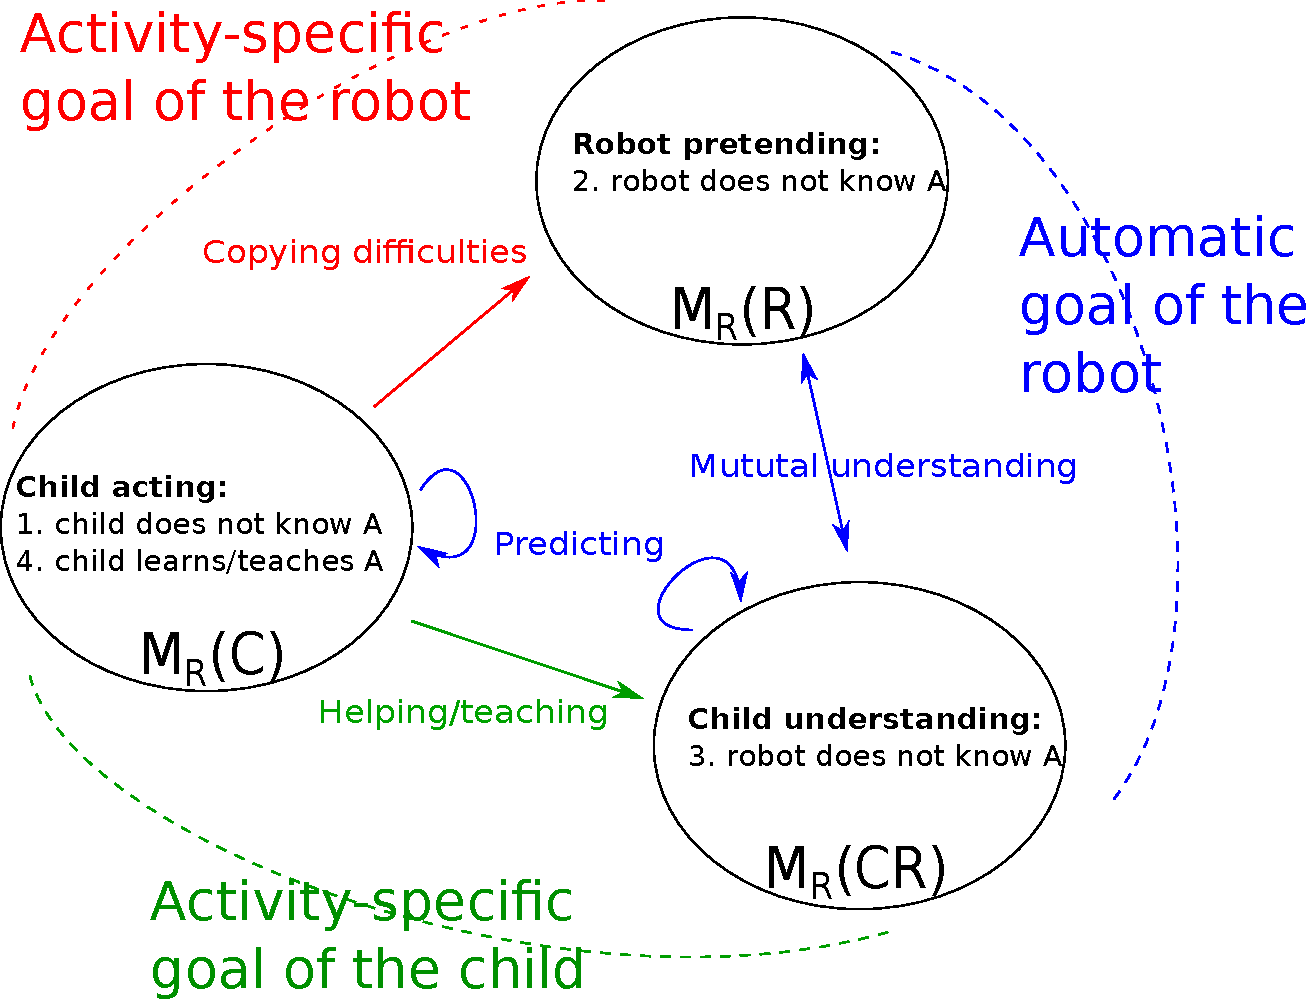
\includegraphics[width=1\columnwidth]{mutual_behaviour}
\caption{\small\textbf{}  }
\label{mm}
\end{figure} 

\section{Repairing miss-understandings}
If an important miss-understanding is detected (given a knowledge $K$, $M_\textit{R}(K) \neq M_\textit{CR}(K)$) the robot can ``turn the tide" of the dynamics between models to figure out what action of the robot leads the child to think that the robot does know $K$, and then exaggerate the action.



\bibliographystyle{IEEEtran}

\bibliography{biblio}

\end{document}


